% section52.tex

%%%%%% Section %%%%%%

\section{\caseENGRUS{Categories of functors}{ / }{Категории функторов}}

For any two categories $\mcC$ and $\mcD$,
\footnote{Technically $\mcC$ has to be small (see Remark \ref{rmk:small}), but as we said there, we are not worrying about that distinction in this book.}
we discussed the category $\Fun(\mcC,\mcD)$ of functors and natural transformations between them. In this section we discuss functor categories a bit more and give some important applications within mathematics (sheaves) that extend to the real world.

%%%% Subsection %%%%

\subsection{\caseENGRUS{Set-valued functors}{ / }{Функторы со значениями в $\Set$}}

Let $\mcC$ be a category. Then we have been writing $\mcC\set$ to denote the functor category $\Fun(\mcC,\Set)$. Here is a nice result about these categories.

\begin{proposition}\label{prop:inst closed under colim lim}

Let $\mcC$ be a category. The category $\mcC\set$ is closed under colimits and limits.

\end{proposition}

\begin{proof}[Sketch of proof]

Let $J$ be an indexing category and $D\taking J\to\mcC\set$ a functor. For each object $c\in\Ob(\mcC)$, we have a functor $D_c\taking J\to\Set$ defined by $D_c(j)=D(j)(c)$. Define a functor $L\taking\mcC\to\Set$ by $L(c)=\lim_J D_c$, and note that for each $f\taking c\to c'$ in $\mcC$ there is an induced function $L(f)\taking L(c)\to L(c')$. One can check that $L$ is a limit of $J$, because it satisfies the relevant universal property. 

The dual proof holds for colimits.

\end{proof}

\begin{application}

When taking in data about a scientific subject, one often finds that the way one thinks about the problem changes over time. We understand this phenomenon in the language of databases in terms of a \href{http://en.wikipedia.org/wiki/Schema_evolution}{\text series of schemas} $\mcC_1,\mcC_2,\ldots,\mcC_n$, perhaps indexed chronologically. The problem is that old data is held in old schemas and we want to see it in our current understanding. The first step is to transfer all the old data to our new schema in the freest possible way, that is, making no assumptions about how to fill in the new fields. If one creates functors $F_i\taking\mcC_i\to\mcC_{i+1}$ from each of these schemas to the next, then we can push the data forward using $\Sigma_{F_i}$. 

Doing this we will have $n$ datasets on $\mcD:=\mcC_n$, namely one for each “epoch of understanding”. Since the category $\mcD\set$ has all colimits, we can take the union of these datasets and get one. It will have many Skolem variables (see Example \ref{ex:left pushforward and skolem}), and these need to be handled in a coherent way. However, the universality of left adjoints could be interpreted as saying that any reasonable formula for handling this old data can be applied to our results.

\end{application}

\begin{exercise}\label{exc:universal objects in C-set}\index{initial object!in $\mcC\set$}\index{terminal object!in $\mcC\set$}
By Proposition \ref{prop:inst closed under colim lim}, the category $\mcC\set$ is closed under taking limits. By Exercises \ref{exc:terminal as limit} and \ref{exc:initial as colimit}, this means in particular that $\mcC\set$ has an initial object and a terminal object. 
\sexc Let $A\in\Ob(\mcC\set)$ be the initial object, considered as a functor $A\taking\mcC\to\Set$. For any $c\in\Ob(\mcC)$, what is the set $A(c)$?
\item Let $Z\in\Ob(\mcC\set)$ be the terminal object, considered as a functor $Z\taking\mcC\to\Set$. For any $c\in\Ob(\mcC)$, what is the set $Z(c)$?
\endsexc
\end{exercise}

Proposition \ref{prop:inst closed under colim lim} says that we can add or multiply database states together. In fact, database states on $\mcC$ form what is called a {\em topos} which means that just about every consideration we made for sets holds for instances on any schema. Perhaps the simplest schema is $\mcC=\fbox{$\bullet$}$, on which the relevant topos is indeed $\Set$. But schemas can be arbitrarily complex, and it is impressive that all of these considerations make sense in such generality. Here is a table that makes a comparison between these domains.
\begin{center}
\begin{tabular}{| l | l |}\bhline
\multicolumn{2}{| c |}{Dictionary between $\Set$ and $\mcC\set$}\\\hline
{\bf Concept in $\Set$}&{\bf Concept in $\mcC\set$}\\\bbhline
Set & Object in $\mcC\set$\\\hline
Function & Morphism in $\mcC\set$\\\hline
Element&Representable functor\\\hline
Empty set & Initial object\\\hline
Natural numbers&Natural numbers object\\\hline
Image&Image\\\hline
(Co)limits&(Co)limits\\\hline
Exponential objects&Exponential objects\\\hline
“Familiar” arithmetic&“Familiar” arithmetic\\\hline
Power sets $2^X$&Power objects $\Omega^X$\\\hline
Characteristic functions&Characteristic morphisms\\\hline
Surjections, injections&Epimorphisms, monomorphisms\\\bhline
\end{tabular}
\end{center}

In the above table we said that elements of a set are akin to representable functors in $\mcC\set$, but we have not yet defined those; we do so in Section \ref{sec:representable functors}. First we briefly discuss monomorphisms and epimorphisms in general (Definition \ref{def:mono, epi}) and then in $\mcC\set$ (Proposition \ref{prop:epi mono in c-set}). 

\begin{definition}[Monomorphism, Epimorphism]\label{def:mono, epi}\index{epimorphism}\index{monomorphism}

Let $\mcS$ be a category and let $f\taking X\to Y$ be a morphism. We say that $f$ is a {\em monomorphism} if it has the following property. For all objects $A\in\Ob(\mcS)$ and morphisms $g,g'\taking A\to X$ in $\mcS$, 
$$
\xymatrix{A\ar@/^1pc/[r]^g\ar@/_1pc/[r]_{g'}&X\ar[r]^f&Y}
$$
if $f\circ g=f\circ g'$ then $g=g'$.

We say that $f\taking X\to Y$ is an {\em epimorphism} if it has the following property. For all objects $B\in\Ob(\mcS)$ and morphisms $h,h'\taking Y\to B$ in $\mcS$,
$$
\xymatrix{X\ar[r]^f&Y\ar@/^1pc/[r]^h\ar@/_1pc/[r]_{h'}&B}
$$
if $h\circ f=h'\circ f$ then $h=h'$.

\end{definition}

In the category of sets, monomorphisms are the same as injections and epimorphisms are the same as surjections (see Proposition \ref{prop:inj and surj}). The same is true in $\mcC\set$: one can check “table by table” that a morphism of instances is mono or epi.

\begin{proposition}\label{prop:epi mono in c-set}

Let $\mcC$ be a category and let $X,Y\taking\mcC\to\Set$ be objects in $\mcC\set$ and let $f\taking X\to Y$ be a morphism in $\mcC\set$. Then $f$ is a monomorphism (respectively an epimorphism) if and only if, for every object $c\in\Ob(\mcC)$, the function $f(c)\taking X(c)\to Y(c)$ is injective (respectively surjective). 

\end{proposition}

\begin{proof}[Sketch of proof]

We first show that if $f$ is mono (respectively epi) then so is $f(c)$ for all $c\in\Ob(\mcC)$. Considering $c$ as a functor $c\taking\ul{1}\to\mcC$, this result follows from the fact that $\Delta_c$ preserves limits and colimits, hence monos and epis. 

We now check that if $f(c)$ is mono for all $c\in\Ob(\mcC)$ then $f$ is mono. Suppose that $g,g'\taking A\to X$ are morphisms in $\mcC\set$ such that $f\circ g=f\circ g'$. Then for every $c$ we have $f\circ g(c)=f\circ g'(c)$ which implies by hypothesis that $g(c)=g'(c)$. But the morphisms in $\mcC\set$ are natural transformations, and if two natural transformations $g,g'$ have the same components then they are the same. 

A similar argument works to show the analogous result for epimorphisms.

\end{proof}

%% Subsubsection %%

\subsubsection{\caseENGRUS{Representable functors}{ / }{Представимые функторы}}\label{sec:representable functors}

Given a category $\mcC$, there are certain functors $\mcC\to\Set$ that come with the package, one for every object in $\mcC$. So if $\mcC$ is a database schema, then for every table $c\in\Ob(\mcC)$ there is a certain database instance associated to it. These instances, i.e. set-valued functors, are called representable functors, and they'll be defined in Definition \ref{def:representable functor}. The idea is that if a database schema represents a conceptual layout of types (e.g. as an olog), then each type $T$ has an instance associated to it, standing for “the generic thing of type $T$ with all its generic attributes”.

\begin{definition}\label{def:representable functor}\index{functor!representable}\index{representable functor}

Let $\mcC$ be a category and let $c\in\Ob(\mcC)$ be an object. The functor $\Hom_\mcC(c,-)\taking\mcC\to\Set$, sending $d\in\Ob(\mcC)$ to the set $\Hom_\mcC(c,d)$ and acting similarly on morphisms $d\to d'$, is said to be {\em represented by $c$}. If a functor $F\taking\mcC\to\Set$ is isomorphic to $\Hom_\mcC(c,-)$, we say that $F$ is {\em a representable functor}. We sometimes write $Y_c:=\Hom_\mcC(c,-)$ for short.

\end{definition}

\begin{example}

Given a category $\mcC$ and an object $c\in\Ob(\mcC)$, we get a representable functor. If we think of $\mcC$ as a database schema and $c$ as a table, then what does the representable functor $Y_c\taking\mcC\to\Set$ look like in terms of databases? It turns out that the following procedure will generate it. 

Begin by writing a new row, say “$\smiley$”, in the ID column of table $c$. For each foreign key column $f\taking c\to c'$, add a row in the ID column of table $c'$ called $“f(\smiley)”$ and record that result (i.e. “$f(\smiley)$”) in the $f$ column of table $c$. Repeat as follows: for each table $d$, identify all rows $r$ that have blank cell in column $g\taking d\to e$. Add a new row called $“g(r)”$ to table $e$ and record that result in the $(r,g)$ cell of table $d$.

Here is a concrete example. Let $\mcC$ be the following schema: 
$$\xymatrix{\LMO{A}\ar[r]^f&\LMO{B}\ar@<.5ex>[r]^{g_1}\ar@<-.5ex>[r]_{g_2}\ar[d]_h&\LMO{C}\ar[r]^i&\LMO{D}\\&\LMO{E}}$$
Then $Y_B\taking\mcC\to\Set$ is the following instance
\begin{center}
\begin{tabular}{| l || l |}\bhline
\multicolumn{2}{|c|}{A}\\\bhline
{\bf ID}&{\bf $f$}\\\bbhline
\end{tabular}
\hsp
\begin{tabular}{| l || l | l | l |}\bhline
\multicolumn{4}{|c|}{B}\\\bhline
{\bf ID}&{\bf $g_1$}&{\bf $g_2$}&{\bf $h$}\\\bbhline
$\smiley$&$g_1(\smiley)$&$g_2(\smiley)$&$h(\smiley)$\\\bhline
\end{tabular}
\hsp
\begin{tabular}{| l || l |}\bhline
\multicolumn{2}{|c|}{C}\\\bhline
{\bf ID}&{\bf $i$}\\\bbhline
$g_1(\smiley)$&$i(g_1(\smiley))$\\\hline
$g_2(\smiley)$&$i(g_2(\smiley))$\\\bhline
\end{tabular}
\end{center}
\begin{center}
\begin{tabular}{| l ||}\bhline
\multicolumn{1}{| c |}{D}\\\bhline
{\bf ID}\\\bbhline
$i(g_1(\smiley))$\\\hline
$i(g_2(\smiley))$\\\bhline
\end{tabular}
\hsp
\begin{tabular}{| l ||}\bhline
\multicolumn{1}{| c |}{E}\\\bhline
{\bf ID}\\\bbhline
$h(\smiley)$\\\bhline
\end{tabular}
\end{center}

We began with a single element in table $B$ and followed the arrows, putting new entries wherever they were required. One might call this the {\em schematically implied reference spread} or {\em SIRS}\index{schematically implied reference spread} of the element $\smiley$ in table $B$. Notice that the table at $A$ is empty, because there are no morphisms $B\to A$.

\end{example}

Representable functors $Y_c$ yield databases states that are as free as possible, subject to having the initial row $\smiley$ in table $c$. We have seen things like this before (by the name of Skolem variables)\index{Skolem} when studying the left pushforward $\Sigma$. Indeed, if $c\in\Ob(\mcC)$ is an object, we can consider it as a functor $c\taking\ul{1}\to\mcC$. A database instance on $\ul{1}$ is the same thing as a set $X$. The left pushforward $\Sigma_c(X)$ has the same kinds of Skolem variables. If $X=\{\smiley\}$ is a one element set, then we get the representable functor $\Sigma_c(\singleton)\iso Y_c$.

\begin{exercise}\label{exc:representables on graph}
Consider the schema for graphs, 
$$\GrIn:=\fbox{\parbox{1in}{\GrInSchema}}$$
\sexc Write down the representable functor $Y_{Ar}\taking\GrIn\to\Set$ as two tables.
\item Write down the representable functor $Y_{V\!e}$ as two tables.
\endsexc
\end{exercise}

\begin{exercise}
Consider the loop schema $$\Loop:=\LoopSchema.$$ What is the representable functor $Y_s\taking\Loop\to\Set$?
\end{exercise}

Let $B$ be a box in an olog, say \fakebox{a person}, and recall that an aspect of $B$ is an outgoing arrow, such as $\fakebox{a person}\To{\tn{has as height in inches}}\fakebox{an integer}$. The following slogan explains representable functors in those terms.

\begin{slogan}
The functor represented by \fakebox{a person} simply leaves a placeholder, like $\la$person's name here$\ra$ or $\la$person's height here$\ra$, for every aspect of \fakebox{a person}. 

In general, there is a representable functor for every type in an olog. The representable functor for type $T$ simply encapsulates the most generic or abstract example of type $T$, by leaving a placeholder for each of its attributes.
\end{slogan}

%% Subsubsection %%

\subsubsection{\caseENGRUS{Yoneda's lemma}{ / }{Лемма Йонеды}}\label{sec:yoneda}

One of the most powerful tools in category theory is Yoneda's lemma. It is often considered by new students to be quite abstract, but grounding it in databases may help.

The idea is this. Suppose that $I\taking\mcC\to\Set$ is a database instance, and let $c\in\Ob(\mcC)$ be an object. Because $I$ is a functor, we know that for every row $r\in I(c)$ in table $c$ a value has been recorded in the $f$-column, where $f\taking c\to c'$ is any outgoing arrow. The value in the $(r,f)$-cell refers to some row in table $c'$. What we're saying is that each row in table $c$ induces SIRS throughout the database. They may not be “Skolem”, or in any sense “freely generated”, but they are there nonetheless. The point is that to each row in $c$ there is a unique mapping $Y_c\to I$. 

\begin{lemma}[Yoneda's lemma, part 1.]\index{Yoneda's lemma}\label{lemma:Yoneda}

Let $\mcC$ be a category, $c\in\Ob(\mcC)$ an object, and $I\taking\mcC\to\Set$ a set-valued functor. There is a natural bijection $$\Hom_{\mcC\set}(Y_c,I)\Too{\iso}I(c).$$

\end{lemma}

\begin{proof}

See \cite{Mac}.

\end{proof}

\begin{example}\label{ex:yoneda}

Consider the category $\mcC$ drawn below:
$$
\mcC:=\parbox{2.1in}{\fbox{\parbox{2.1in}{\begin{center}\small mother\;$\circ$\;firstChild\;=\;$\id_{\tn{Mother}}$\normalsize\end{center}$$\xymatrix{\LTO{Child}\ar[rr]^{\tn{mother}}&&\LTO{Mother}\ar@/^1pc/[ll]^{\tn{firstChild}}}$$}}}
$$
There are two representable functors, $Y_{\tt Child}$ and $Y_{\tt Mother}$. The latter, when written as a database instance, will consist of a single row in each table. The former, $Y_{\tt Child}\taking\mcC\to\Set$ is shown here:
\begin{center}
\begin{tabular}{| l || l |}\bhline
\multicolumn{2}{|c|}{Child}\\\bhline
{\bf ID}&{\bf mother}\\\hline
$\smiley$&mother($\smiley$)\\\hline
firstChild(mother($\smiley$))&mother($\smiley$)\\\bbhline
\end{tabular}
\hsp
\begin{tabular}{| l || l |}\bhline
\multicolumn{2}{|c|}{Mother}\\\bhline
{\bf ID}&{\bf firstChild}\\\bbhline
mother($\smiley$)&firstChild(mother($\smiley$))\\\bhline
\end{tabular}
\end{center}
The representable functor $Y_{\tt Child}$ is the freest instance possible, starting with one element in the Child table and satisfying the constraints. 

Here is another instance $I\taking\mcC\to\Set$:
\begin{center}
\begin{tabular}{| l || l |}\bhline
\multicolumn{2}{|c|}{\tt Child}\\\bhline
{\bf ID}&{\bf mother}\\\hline
Amy&Ms. Adams\\\hline
Bob&Ms. Adams\\\hline
Carl&Ms. Jones\\\hline
Deb&Ms. Smith\\\bhline
\end{tabular}
\hsp
\begin{tabular}{| l || l |}\bhline
\multicolumn{2}{|c|}{\tt Mother}\\\bhline
{\bf ID}&{\bf firstChild}\\\bbhline
Ms. Adams&Bob\\\hline
Ms. Jones&Carl\\\hline
Ms. Smith&Deb\\\bhline
\end{tabular}
\end{center}

\end{example}

Yoneda's lemma (\ref{lemma:Yoneda}) is about the set of natural transformations $Y_{\tt Child}\to I$. Recall from Definition \ref{def:natural transformation} that a search for natural transformations can get a bit tedious. Yoneda's lemma makes the calculation quite trivial. In our case there are exactly four such natural transformations, and they are completely determined by where $\smiley$ goes. In some sense the symbol $\smiley$ {\em represents} child-ness in our database. 

\begin{exercise}
Consider the schema $\mcC$ and instance $I\taking\mcC\to\Set$ from Example \ref{ex:yoneda}. Let $Y_{\tt Child}$ be the representable functor as above. 
\sexc Let $\alpha\taking Y_{\tt Child}\to I$ be the natural transformation sending $\smiley$ to Amy. What is $\alpha_{\tn{Child}}(\tn{firstChild(mother}(\smiley)))$?
\footnote{There is a lot of clutter, perhaps. Note that “firstChild(mother($\smiley$))” is a row in the {\tt Child} table. Assuming that the math follows the meaning, if $\smiley$ points to Amy, where should firstChild(Mother($\smiley$)) point?}
\item Let $\alpha\taking Y_{\tt Child}\to I$ be the natural transformation sending $\smiley$ to Bob. What is $\alpha_{\tt Child}(\tn{firstChild(mother}(\smiley)))$?
\item Let $\alpha\taking Y_{\tt Child}\to I$ be the natural transformation sending $\smiley$ to Carl. What is $\alpha_{\tt Child}(\tn{firstChild(mother}(\smiley)))$?
\item Let $\alpha\taking Y_{\tt Child}\to I$ be the natural transformation sending $\smiley$ to Deb. What is $\alpha_{\tt Child}(\tn{firstChild(mother}(\smiley)))$?
\item Let $\alpha\taking Y_{\tt Child}\to I$ be the natural transformation sending $\smiley$ to Amy. What is $\alpha_{\tt Mother}(\tn{mother}(\smiley))$?
\endsexc
\end{exercise}

We saw in Section \ref{sec:representable functors} that a representable functor is a mathematically-generated database instance for an abstract thing of type $T$. It creates placeholders for every attribute that things of type $T$ are supposed to have.

\begin{slogan}
Yoneda's lemma says the following. Specifying an actual thing of type $T$ is the same as filling in all placeholders found in the generic thing of type $T$.
\end{slogan}

Yoneda's lemma is considered by many category theory lovers to be the most important tool in the subject. While its power is probably unclear to students whose sole background in category theory comes from this book, Yoneda's lemma is indeed extremely useful for reasoning. It allows us to move the notion of functor application into the realm of morphisms between functors (i.e. morphisms in $\mcC\set$, which are natural transformations). This keeps everything in one place — it's all in the morphisms — and thus more interoperable.

\begin{example}\label{ex:yoneda for cyclic monoid}

In Example \ref{ex:cyclic monoid (7,4)}, we discussed the cyclic monoid $\mcM$ generated by the symbol $Q$ and subject to the relation $Q^7=Q^4$. We drew a picture like this: 
\begin{align}\label{dia:grothendieck yoneda (4,7)}
\xymatrix@=15pt{
\LMO{Q^0}\ar[rr]&&\LMO{Q^1}\ar[rr]&&\LMO{Q^2}\ar[rr]&&\LMO{Q^3}\ar[rr]&&\LMO{Q^4}\ar[dr]\\
&&&&&&&\LMO{Q^6}\ar[ur]&&\LMO{Q^5}\ar[ll]
}
\end{align}
We are finally ready to give the mathematical foundation for this picture. Since $\mcM$ is a category with one object, $\monOb$, there is a unique representable functor (up to isomorphism) $Y:=Y_\monOb\taking\mcM\to\Set$. A functor $\mcM\to\Set$ can be thought of as a set with an $\mcM$-action, as discussed in Section \ref{sec:monoids as cats}. Here the required set is 
$$Y(\monOb)=\Hom_\mcM(\monOb,\monOb)\iso\{Q^0,Q^1,Q^2,Q^3,Q^4,Q^5,Q^6\}$$ 
and the action is pretty straightforward (it is called the {\em principal action}). We might say that (\ref{dia:grothendieck yoneda (4,7)}) is a picture of this principal action of $\mcM$. 

However, we can go one step further. Given a functor $Y\taking\mcM\to\Set$, we can take its category of elements, $\int_\mcM Y$ as in Section \ref{sec:grothendieck construction}. The category $\int_\mcM Y$ has objects $Y(\monOb)\in\Ob(\Set)$, i.e. the set of dots in (\ref{dia:grothendieck yoneda (4,7)}), and it has a unique morphism $Q^i\to Q^j$ for every path of length $\leq 6$ from $Q^i$ to $Q^j$ in that picture.

\end{example}

\begin{exercise}

Let $c\in\Ob(\mcC)$ be an object and let $I\in\Ob(\mcC\set)$ be another object. Consider $c$ also as a functor $c\taking\ul{1}\to\mcC$ and recall the pullback functor $\Delta_c\taking\mcC\set\to\Set$ and its left adjoint $\Sigma_c\taking\Set\to\mcC\set$ from Section \ref{sec:data migration}.
\sexc What is the set $\Delta_c(I)$?
\item What is $\Hom_\Set(\singleton,\Delta_c(I))$?
\item What is $\Hom_{\mcC\set}(\Sigma_c(\singleton),I)$?
\item How does $\Sigma_c(\singleton)$ compare to $Y_c$, the functor represented by $c$, as objects in $\mcC\set$?
\endsexc
\end{exercise}

\begin{lemma}[Yoneda's lemma, part 2]

Let $\mcC$ be a category. The assignment $c\mapsto Y_c$ from Lemma \ref{lemma:Yoneda} extends to a functor $Y\taking\mcC\op\to\mcC\set$, and this functor is fully faithful. 

In particular, if $c,c'\in\Ob(\mcC)$ are objects and there is an isomorphism $Y_c\iso Y_{c'}$ in $\mcC\set$, then there is an isomorphism $c\iso c'$ in $\mcC$.

\end{lemma}
\begin{proof}
See \cite{Mac}.
\end{proof}

\begin{exercise}
The distributive law for addition of natural numbers says $(a+b)\times c=a\times c+b\times c$. Below we will give a proof of the distributive law, using category-theoretic reasoning. Annotate anything in {\color{red}red} ink  with a justification for why it is true.
\begin{proposition}
For any natural numbers $a,b,c\in\NN$, the distributive law 
$$(a+b)c=ac+bc$$ 
holds.
\end{proposition}
\begin{proof}[Sketch of proof. To finish, justify {\color{red}red stuff}]
~\\
Let $A,B,C$ be finite sets and let $X$ be another finite set.
\begin{align*}
\Hom_\Set((A+B)\times C,X)
&{\color{red}\iso}\Hom_\Set(A+B,X^C)\\
&{\color{red}\iso}\Hom_\Set(A,X^C)\times\Hom_\Set(B,X^C)\\
&{\color{red}\iso}\Hom_\Set(A\times C,X)\times\Hom_\Set(B\times C,X)\\
&{\color{red}\iso}\Hom_\Set((A\times C)+(B\times C),X).
\end{align*}
By {\color{red} the appropriate application} of Yoneda's lemma, we see that there is an isomorphism
$$(A+B)\times C\iso(A\times C)+(B\times C)$$
in $\Fin$. The result about natural numbers {\color{red}follows}.
\end{proof}
\end{exercise}



%% Subsubsection %%

\subsubsection{\caseENGRUS{The subobject classifier $\Omega\in\Ob(\mcC\set)$}{ / }{Классификатор подобъектов $\Omega\in\Ob(\mcC\set)$}}\index{subobject classifier!in $\mcC\set$}

If $\mcC$ is a category then the functor category $\mcC\set$ is a very nice kind of category, called a {\em topos}.\index{topos} Note that when $\mcC=\ul{1}$ is the terminal category, then we have an isomorphism $\mcC\set\iso\Set$, so the category of sets is a special case of a topos. What is so interesting about toposes (or topoi) is that they so nicely generalize many properties of $\Set$. In this short section we investigate only one such property, namely that $\mcC\set$ has a subobject classifier, denoted $\Omega\in\Ob(\mcC\set)$. In the case $\mcC=\ul{1}$, we saw back in Section \ref{def:subobject classifier} that the subobject classifier is $\{True,False\}\in\Ob(\Set)$. 

As usual, we consider the matter of subobject classifiers by grounding the discussion in terms of databases.

\begin{definition}

Let $\mcC$ be a category, let $\mcC\set$ denote its category of instances, and let $1\in\Ob(\mcC\set)$ denote the terminal object. A {\em subobject classifier for $\mcC\set$} is an object $\Omega_\mcC\in\Ob(\mcC\set)$ and a morphism $t\taking 1\to\Omega_\mcC$ with the following property. For any monomorphism $f\taking X\to Y$ in $\mcC\set$, there exists a unique morphism $char(f)\taking Y\to\Omega_\mcC$ such that the following diagram is a pullback in $\mcC\set$:
$$
\xymatrix@=25pt{X\ar[r]^{!}\ar[d]_f\ullimit&1\ar[d]^t\\Y\ar[r]_{char(f)}&\Omega_\mcC
}
$$

\end{definition}

In terms of databases, what this means is that for every schema $\mcC$ there is some special instance $\Omega_\mcC\in\Ob(\mcC\set)$ that somehow classifies sub-instances. When our schema is the terminal category, $\mcC=\ul{1}$, instances are sets and we saw in Definition \ref{def:subobject classifier} that the subobject classifier is $\Omega_{\ul{1}}=\{True, False\}$. One might think that the subobject classifier for $\mcC\set$ should just consist of a two-element set table-by-table, i.e. that for every $c\in\Ob(\mcC)$ we should have $\Omega_{\mcC}=^?\{True,False\}$, but this is not correct. 

In fact, for any object $c\in\Ob(\mcC)$, it is easy to say what $\Omega_\mcC(c)$ should be. We know by Yoneda's lemma (Lemma \ref{lemma:Yoneda}) that $\Omega_\mcC(c)=\Hom_{\mcC\set}(Y_c,\Omega_\mcC)$, where $Y_c$ is the functor represented by $c$. There is a bijection between $\Hom_{\mcC\set}(Y_c,\Omega_\mcC)$ and the set of sub-instances of $Y_c$. Each morphism $f\taking c\to d$ in $\mcC$ induces a morphism $Y_f\taking Y_d\to Y_c$, and the map $\Omega_\mcC(f)\taking\Omega_\mcC(c)\to\Omega_\mcC(d)$ sends a sub-instance $A\ss Y_c$ to the pullback 
$$
\xymatrix{Y_f^\m1(A)\ar[r]\ar[d]\ullimit&A\ar[d]\\Y_d\ar[r]_{Y_f}&Y_c}
$$

But this is all very abstract. We now give an example of a subobject classifier.  

\begin{example}

Consider the category $\mcC\iso[3]$ depicted below
$$\mcC:=\parbox{3in}{\fbox{
\xymatrix{&&&\ar@{}[d]|(.4){\checkmark}&&&\\
\LTO{0}\ar[rr]^{\tn{after\_1}}\ar@/_1.5pc/[rrrr]_{\tn{after\_2}}\ar@/^3pc/[rrrrrr]^{\tn{after\_3}}&&\LTO{1}\ar[rr]^{\tn{after\_1}}\ar@/_1.5pc/[rrrr]_{\tn{after\_2}}&&\LTO{2}\ar[rr]^{\tn{after\_1}}&&\LTO{3}\\
&&&\ar@{}[ull]|(.8){\checkmark}\ar@{}[urr]|(.8){\checkmark}&&
}}}
$$
To write down $\Omega_\mcC$ we need to understand the representable functors $Y_c\in\Ob(\mcC\set)$, for $c={\tt 0},{\tt 1},{\tt 2},{\tt 3}$, as well as their subobjects. Here is $Y_{\tt 0}$ as an instance:

\begin{center}\small
\begin{tabular}{| l || l | l | l |}
\bhline
\multicolumn{4}{|c|}{$Y_{\tt 0}({\tt 0})$}\\\bhline
{\bf ID}&{\bf after\_1}&{\bf after\_2}&{\bf after\_3}\\\bbhline
$\smiley$&after\_1($\smiley$)&after\_2($\smiley$)&after\_3($\smiley$)\\\bhline
\end{tabular}
\hsp
\begin{tabular}{| l || l | l |}
\bhline
\multicolumn{3}{|c|}{$Y_{\tt 0}({\tt 1})$}\\\bhline
{\bf ID}&{\bf after\_1}&{\bf after\_2}\\\bbhline
after\_1$(\smiley)$&after\_2$(\smiley)$&after\_3$(\smiley)$\\\bhline
\end{tabular}\\\vspace{.2in}
\begin{tabular}{| l || l |}
\bhline
\multicolumn{2}{|c|}{$Y_{\tt 0}({\tt 2})$}\\\bhline
{\bf ID}&{\bf after\_1}\\\bbhline
after\_2$(\smiley)$&after\_3$(\smiley)$\\\bhline
\end{tabular}
\hsp
\begin{tabular}{| l ||}
\bhline
\multicolumn{1}{|c|}{$Y_{\tt 0}({\tt 3})$}\\\bhline
{\bf ID}\\\bbhline
after\_3$(\smiley)$\\\bhline
\end{tabular}

\end{center}

What are the sub-instances of this? There is the empty sub-instance $\emptyset\ss Y_{\tt 0}$ and the identity sub-instance $Y_{\tt 0}\ss Y_{\tt 0}$. But there are three more as well. Note that if we want to keep the $\smiley$ row of table {\tt 0} then we have to keep everything. But if we throw away the $\smiley$ row of table {\tt 0} we can still keep the rest and get a sub-instance. If we want to keep the after\_1$(\smiley)$ row of table {\tt 1} then we have to keep its images in tables {\tt 2} and {\tt 3}. But we could throw away both the $\smiley$ row of table {\tt 0} and the after\_1$(\smiley)$ row of table {\tt 1} and still keep the rest. And so on. In other words, the subobjects of $Y_{\tt 0}$ are in bijection with the set $\Omega_\mcC({\tt 0}):=\{\tn{{\it yes}, {\it in 1}, {\it in 2}, {\it in 3}, {\it never}}\}$. 

The same analysis holds for the other tables of $\Omega_\mcC$. It looks like this:
\begin{center}
\begin{tabular}{| l || l | l | l |}
\bhline
\multicolumn{4}{|c|}{$\Omega_\mcC({\tt 0})$}\\\bhline
{\bf ID}&{\bf after\_1}&{\bf after\_2}&{\bf after\_3}\\\bbhline
{\it yes}&{\it yes}&{\it yes}&{\it yes}\\\hline
{\it in 1}&{\it yes}&{\it yes}&{\it yes}\\\hline
{\it in 2}&{\it in 1}&{\it yes}&{\it yes}\\\hline
{\it in 3}&{\it in 2}&{\it in 1}&{\it yes}\\\hline
{\it never}&{\it never}&{\it never}&{\it never}\\\bhline
\end{tabular}
\hsp
\begin{tabular}{| l || l | l |}
\bhline
\multicolumn{3}{|c|}{$\Omega_\mcC({\tt 1})$}\\\bhline
{\bf ID}&{\bf after\_1}&{\bf after\_2}\\\bbhline
{\it yes}&{\it yes}&{\it yes}\\\hline
{\it in 1}&{\it yes}&{\it yes}\\\hline
{\it in 2}&{\it in 1}&{\it yes}\\\hline
{\it never}&{\it never}&{\it never}\\\bhline
\end{tabular}\\\vspace{.2in}
\begin{tabular}{| l || l |}
\bhline
\multicolumn{2}{|c|}{$\Omega_\mcC({\tt 2})$}\\\bhline
{\bf ID}&{\bf after\_1}\\\bbhline
{\it yes}&{\it yes}\\\hline
{\it in 1}&{\it yes}\\\hline
{\it never}&{\it never}\\\bhline
\end{tabular}
\hsp
\begin{tabular}{| l ||}
\bhline
\multicolumn{1}{|c|}{$\Omega_\mcC({\tt 3})$}\\\bhline
{\bf ID}\\\bbhline
{\it yes}\\\hline
{\it never}\\\bhline
\end{tabular}

\end{center}
The morphism $1\to\Omega_\mcC$ picks out the {\it yes} row of every table.

Now that we have constructed $\Omega_\mcC\in\Ob(\mcC\set)$, we are ready to see it in action. What makes $\Omega_\mcC$ special is that for any instance $X\taking\mcC\to\Set$, the subinstances if $X$ are in one-to-one correspondence with the morphisms $X\to\Omega_\mcC$. Consider the following arbitrary instance $X$, where the blue rows denote a sub-instance $A\ss X$.

\begin{align}\label{dia:instance for omega}\footnotesize
\begin{array}{| l || l | l | l |}
\bhline
\multicolumn{4}{|c|}{X({\tt 0})}\\\bhline
{\bf ID}&{\bf after\ 1}&{\bf after\ 2}&{\bf after\ 3}\\\bbhline
a_1&b_1&\color{blue}{c_1}&\color{blue}{d_1}\\\hline
a_2&\color{blue}{b_2}&\color{blue}{c_1}&\color{blue}{d_1}\\\hline
a_3&\color{blue}{b_2}&\color{blue}{c_1}&\color{blue}{d_1}\\\hline
a_4&b_3&c_2&d_2\\\hline
a_5&b_5&c_3&\color{blue}{d_1}\\\bhline
\end{array}
\hspace{.2in}
\begin{array}{| l || l | l |}
\bhline
\multicolumn{3}{|c|}{X({\tt 1})}\\\bhline
{\bf ID}&{\bf after\ 1}&{\bf after\ 2}\\\bbhline
b_1&\color{blue}{c_1}&\color{blue}{d_1}\\\hline
\color{blue}{b_2}&\color{blue}{c_1}&\color{blue}{d_1}\\\hline
b_3&c_2&d_2\\\hline
\color{blue}{b_4}&\color{blue}{c_1}&\color{blue}{d_1}\\\hline
b_5&c_3&\color{blue}{d_1}\\\bhline
\end{array}\hspace{.2in}
\begin{array}{| l || l |}
\bhline
\multicolumn{2}{|c|}{X({\tt 2})}\\\bhline
{\bf ID}&{\bf after\ 1}\\\bbhline
\color{blue}{c_1}&\color{blue}{d_1}\\\hline
c_2&d_2\\\hline
c_3&\color{blue}{d_1}\\\bhline
\end{array}
\hspace{.2in}
\begin{array}{| l ||}
\bhline
\multicolumn{1}{|c|}{X({\tt 3})}\\\bhline
{\bf ID}\\\bbhline
\color{blue}{d_1}\\\hline
d_2\\\bhline
\end{array}
\end{align}

This blue sub-instance $A\ss X$ corresponds to a map $char(A)\taking X\to\Omega_\mcC$. That is for each $c\in\Ob(\mcC)$ the rows in the $c$-table of $X$ are sent to the rows in the $c$-table of $\Omega_\mcC$. The way $char(A)$ works is as follows. For each table $i$ and row $x\in X(i)$, find the first column $f$ in which the entry is blue (i.e. $f(x)\in A$), and send $x$ to the corresponding element of $\Omega_\mcC(i)$. For example, $char(A)({\tt 0})$ sends $a_1$ to {\it in 2} and sends $a_4$ to {\it never}, and $char(A)({\tt 2})$ sends $c_1$ to {\it yes} and sends $c_2$ to {\it never}.

\end{example}

\begin{exercise}
\sexc Write out the blue subinstance $A\ss X$ shown in (\ref{dia:instance for omega}) as an instance of $\mcC$, i.e. as four tables. 
\item This subinstance $A\ss X$ corresponds to a map $\ell:=char(A)\taking X\to\Omega_\mcC$. For all $c\in\Ob(\mcC)$ we have a function $\ell(c)\taking X(c)\to\Omega_\mcC(c)$. With $c={\tt 1}$, write out $\ell({\tt 1})\taking X({\tt 1})\to\Omega_\mcC({\tt 1})$.
\endsexc
\end{exercise}

\begin{exercise}
Let $\Loop$ be the loop schema 
$$\Loop=\LoopSchema.$$ 
\sexc What is the subobject classifier $\Omega_\Loop\in\Ob(\Loop\set)$?
\item How does $\Omega_\Loop$ compare to the representable functor $Y_s$?
\endsexc
\end{exercise}

\begin{exercise}   
Let $\GrIn=\fbox{\GrInSchema}$ be the indexing category for graphs. 
\sexc Write down the subobject classifier $\Omega_\GrIn\in\Ob(\GrIn\set)$ in tabular form, i.e. as two tables.
\item Draw $\Omega_\GrIn$ as a graph.
\item Let $G$ be the graph below and $G'\ss G$ the blue part.
$$\xymatrix{
\LMO{\color{blue}{w}}\ar@/^1pc/[r]^f\ar@[blue][r]_{\color{blue}{g}}\ar[d]_h&\LMO{\color{blue}{x}}\\
\LMO{y}\ar@(l,d)[]_j\ar[r]_i&\LMO{\color{blue}{z}}
}
$$
Write down $G\in\Ob(\GrIn\set)$ in tabular form.
\item Write down the components of the natural transformation $char(G')\taking G\to\Omega_\GrIn$.
\endsexc
\end{exercise}

%%%% Subsection %%%%

\subsection{\caseENGRUS{Database instances in other categories}{ / }{Экземпляры баз данных в других категориях}}

%% Subsubsection %%

\subsubsection{\caseENGRUS{Representations of groups}{ / }{Представления групп}}\label{ex:reps of groups}

The classical mathematical subject of {\em representation theory}\index{representation theory} is the study of $\Fun(G,\Vect)$ where $G$ is a group and $\Vect$ is the category of vector spaces (over say $\RR$).\index{vector space}\index{a category!$\Vect$} Every such functor $F\taking G\to\Vect$ is called a {\em representation of $G$}. Since $G$ is a category with one object $\monOb$, $F$ consists of a single vector space $V=F(\monOb)$ together with an action of $G$ on it. 

We can think of this in terms of databases if we have a presentation of $G$ in terms of generators and relations. The schema corresponding to $G$ has one table and this table has a column for each generator. Giving a representation $F$ is the same as giving an instance on our schema, with some properties that stem from the fact that our target category is $\Vect$ rather than $\Set$. There are many possibilities for expressing
\footnote{We would use the term “representing” or “presenting”, but they are both taken in the context of our narrative!}
such data.

One possibility is if we could somehow draw $V$, say if $V$ is 1-, 2-, or 3-dimensional. If so, let $P$ be our chosen picture of $V$, e.g. $P$ is the standard drawing of a Cartesian coordinate plane. Then every column of our table would consist entirely of the picture $P$ instead of a set of rows. Drawing a point in the ID-column picture would result in a point being drawn in each other column's picture, in accordance with the $G$-action. Each column would of course respect addition and scalar multiplication.

Another possibility is to use the fact that there is a functor $U\taking\Vect\to\Set$, so our instance $F\taking G\to\Vect$ can be converted to an ordinary instance $U\circ F\taking G\to\Set$. We would have an ordinary set of rows. This set would generally be infinite, but it would be structured by addition and scalar multiplication. For example, assuming $V$ is finite dimensional, one could find a few rows that generated the rest. 

A third possibility is to use monads, which allow the table to have only as many rows as $V$ has dimensions. This is a considerable savings of space. See Section \ref{sec:monads}.

%% Subsubsection %%

\subsubsection{\caseENGRUS{Representations of quivers}{ / }{Представления колчанов}}

Representation theory also studies representations of quivers. A {\em quiver} is just the free category (see Example \ref{ex:free category}\index{category!free category}\index{graph!free category on}) on a graph. If $P$ is a graph with free category $\mcP$ then a representation of the quiver $\mcP$ is a functor $F\taking\mcP\to\Vect$. Such a representation consists of a vector space at every vertex of $P$ and a linear transformation for every arrow. All of the discussion from Section \ref{ex:reps of groups} works in this setting, except that there is more than one table.

%% Subsubsection %%

\subsubsection{\caseENGRUS{Other target categories}{ / }{Другие категории в качестве области значений}}\label{sec:other targets}

One can imagine the value of using target categories other than $\Set$ or $\Vect$ for databases. 

\begin{application}\index{geography}

\href{http://en.wikipedia.org/wiki/Geographic_data}{\text Geographic data} consists of maps of the earth together with various functions on it. For example for any point on the earth one may want to know the average temperature recorded in the past 10 years, or the precise temperature at this moment. Earth can be considered as a topological space, $E$. Similarly, temperatures on earth reside on a continuum, say the space $T$ of real numbers $[-100,200]$. Thus the temperature record is a function $E\to T$. 

Other records such as precipitation, population density, elevation, etc. can all be considered as continuous functions from $E$ to some space. Agencies like the US Geological Survey hold databases of such information. By modeling them on functors $\mcC\to\Top$, they may be able to employ mathematical tools such as persistent homology \cite{WeS} to find interesting invariants of the data.

\end{application}

\begin{application}

Many other scientific disciplines could use the same kind of tool. For example, in studying the \href{http://en.wikipedia.org/wiki/Strength_of_materials}{\text mechanics of materials}, one may want to consider the material as a topological space $M$ and measure values such as energy as a continuous $M\to E$. Such observations could be modeled by databases with target category $\Top$ or $\Vect$ rather than $\Set$.

\end{application}

%%%% Subsection %%%%

\subsection{\caseENGRUS{Sheaves}{ / }{Пучки}}\label{sec:sheaves}\index{sheaves}

Let $X$ be a topological space (see Example \ref{ex:topological space}), such as a sphere. In Section \ref{sec:other targets} we discussed continuous functions out of $X$, and their use in science (e.g. recording temperatures on the earth as a continuous map $X\to[-100,200]$). Sheaves allow us to consider the local-global nature of such maps, taking into account reparable discrepancies in data gathering tools. 

\begin{application}\label{app:sheaves of temperature}

Suppose that $X$ is the topological space corresponding to the earth; by a {\em region} we mean an open subset $U\ss X$. Suppose that we cover $X$ with 10,000 regions $U_1,U_2,\ldots,U_{10000}$, such that some of the regions overlap in a non-empty subregion (e.g. perhaps $U_5\cap U_9\neq\emptyset)$. For each $i,j$ let $U_{i,j}=U_i\cap U_j$. 

For each region $U_i\ss X$ we have a temperature recording device, which gives a function $T_i\taking U_i\to[-100,200]$. If $U_i\cap U_j\neq\emptyset$ then two different recording devices give us temperature data for the intersection $U_{i,j}$. Suppose we find that they do not give precisely the same data, but that there is a translation formula between their results. For example, $T_i$ might register $3^\circ$ warmer than $T_j$ registers, throughout the region $U_i\cap U_j$.

A consistent system of translation formulas is called a {\em sheaf}. It does not demand a universal “true” temperature function, but only a consistent translation system between them. 

\end{application}

The following definitions (Definitions \ref{def:presheaf}, \ref{def:sheaf}) make the notion of sheaf precise, but we must go slowly (because it will already feel quick to the novice). For every region $U$, we can record the value of some function (say temperature) throughout $U$; although this record might consist of a mountain of data (a temperature for each point in $U$!), we think of it as one thing. That is, it is one element in the set of value-assignments throughout $U$. A sheaf holds the set of possible values-assignments-throughout-$U$'s for all the different regions $U$, as well as how a value-assignment-throughout-$U$ restricts to a value-assignment-throughout-$V$ for any subset $V\ss U$.

\begin{definition}\label{def:presheaf}\index{presheaf}

Let $X$ be a topological space, let $\Op(X)$ denote its partial order of open sets, and let $\Op(X)\op$ be the opposite category. A {\em presheaf on $X$} is a functor $\mcO\taking\Op(X)\op\to\Set$. For every open set $U\ss X$ we refer to the set $\mcO(U)$ as the {\em set of values-assignments throughout $U$ of $\mcO$}. If $V\ss U$ is an open subset, it corresponds to an arrow in $\Op(X)$ and applying the functor $\mcO$ yields a function called the {\em restriction map from $U$ to $V$} and denoted $\rho_{V,U}\taking\mcO(U)\to\mcO(V)$. Given $a\in\mcO(U)$, we may denote $\rho_{V,U}(a)$ by $a|_V$; it is called {\em the restriction of $a$ to $V$}.

The {\em category of presheaves on $X$} is simply $\Op(X)\op\set$; see Definition \ref{def:mcC-set}.

\end{definition}

\begin{exercise}~
\sexc Come up with $4$ overlapping open subsets that cover the square $X:=[0,3]\times[0,3]\ss\RR^2$. Write down a label for each open set as well as a label for each overlap (2-fold, 3-fold, etc.); you now have labeled $n$ open sets. For each of these open sets, draw a dot with the appropriate label, and then draw an arrow from one dot to another when the first refers to an open subset of the second. This is a preorder; call it $\Op(X)$. Now make up and write down formulas $R_1\taking X\to\RR$ and $R_2\taking X\to\RR$ with $R_1\leq R_2$, expressing a range of temperatures $R_1(p)\leq x\leq R_2(p)$ that an imaginary experiment shows can exist at each point $p$ in the square. 
\item Suppose we now tried to make our presheaf $\mcO\taking\Op(X)\op\to\Set$ as follows. For each of your open sets, say $A$, we could put $$\mcO(A):=\{f\taking A\to\RR\|R_1(a)\leq f(a)\leq R_2(a)\}.$$ What are the restriction maps? Do you like the name “value-assignment throughout $A$” for elements of $\mcO(A)$? 
\item We can now make another presheaf $\mcO'$ given the same experiment. For each of your open sets, say $A$, we could put $$\mcO'(A):=\{f\taking A\to\RR\|f\tn{ is continuous, and }R_1(a)\leq f(a)\leq R_2(a)\}.$$ Are you comfortable with the idea that there is a morphism of presheaves $\mcO'\to\mcO$?
\endsexc
\end{exercise}

Before we define sheaves, we need to clarify the notion of covering. Suppose that $U$ is a region and that $V_1,\ldots,V_n$ are subregions (i.e. for each $1\leq i\leq n$ we have $V_i\ss U$). Then we say that the $V_i$ {\em cover} $U$ if every point in $U$ is in $V_i$ for some $i$. Another way to say this is that the natural function $\sqcup_iV_i\to U$ is surjective.

\begin{example}\label{ex:open cover}\index{open cover}

Let $X=\RR$ be the space of real numbers, and define the following open subsets: $U=(5,10), V_1=(5,7), V_2=(6,9), V_3=(7,10)$.
\footnote{We use parentheses to denote open intervals of real numbers. For example $(6,9)$ denotes the set $\{x\in\RR\|6<x<9\}$.} 
Then $V_1, V_2, V_3$ is a cover of $U$. It has overlaps $V_{12}=V_1\cap V_2=(6,7)$, $V_{13}=V_1\cap V_3=\emptyset$, $V_{23}=V_2\cap V_3=(7,9)$. 

Given a presheaf $\mcO\taking\Op(X)\op\to\Set$, we have sets and functions as in the following (incomplete) diagram
$$
\xymatrix@=15pt{
&&\mcO(V_1)\ar[drr]\\
&&&&\mcO(V_1\cap V_2)\\
\mcO(U)\ar[uurr]\ar[rr]\ar[ddrr]&&\mcO(V_2)\ar[urr]\ar[drr]\\
&&&&\mcO(V_2\cap V_3)\\
&&\mcO(V_3)\ar[urr]
}
$$

\end{example}

A presheaf $\mcO$ on $X$ tells us what value-assignments throughout $U$ can exist for each $U$. Suppose we have a value-assignment $a\in\mcO(U)$ throughout $U$ and another value-assignment $a'\in\mcO(U')$ throughout $U'$, and suppose that they agree as value-assignments throughout $U\cap U'$, i.e. $a|_{U\cap U'}=a'|_{U\cap U'}$. In this case we should have a unique value-assignment $b\in\mcO(U\cup U')$ throughout $U\cup U'$ that agrees on the $U$-part with $a$ and agrees on the $U'$-part with $a'$; i.e. $b|_U=a$ and $b|_{U'}=a'$. This is the sheaf condition. 

\begin{definition}\label{def:sheaf}

Let $X$ be a topological space, let $\Op(X)$ be its partial order of open sets, and let $\mcO\taking\Op(X)\op\to\Set$ be a presheaf. Given an open set $U\ss X$ and a cover $V_1,\ldots, V_n$ of $U$, the following condition is called the {\em sheaf condition}\index{sheaf!condition} for that cover. 
\begin{description}
\item [Sheaf condition] Given a sequence $a_1,\ldots,a_n$ where each is a value-assignment $a_i\in\mcO(V_i)$ throughout $V_i$, suppose that for all $i,j$ we have $a_i|_{V_i\cap V_j}=a_j|_{V_i\cap V_j}$; then there is a unique value-assignment $b\in\mcO(U)$ such that $b|_{V_i}=a_i$.
\end{description}
The presheaf $\mcO$ is called a {\em sheaf} if it satisfies the sheaf condition for every cover.

\end{definition}

\begin{example}

Let $X=\RR$ and let $U, V_1,V_2,V_3$ be the open cover given in Example \ref{ex:open cover}. Given a measurement taken throughout $V_1$, a measurement taken throughout $V_2$, and a measurement taken throughout $V_3$, we have elements $a_1\in\mcO(V_1), a_2\in\mcO(V_2),$ and $a_3\in\mcO(V_3)$. If they are in agreement on the overlap intervals, we can {\em glue} \index{sheaf!glueing} them to give a measurement throughout $U$.

\end{example}

\begin{remark}

In Application \ref{app:sheaves of temperature}, we said that sheaves would help us patch together information from different sources. Even if different temperature-recording devices $T_i$ and $T_j$ registered different temperatures on an overlapping region $U_i\cap U_j$, we said they could be patched together if there was a consistent translation system between their results. What is actually needed is a set of isomorphisms 
$$p_{i,j}\taking T_i|_{U_{i,j}}\To{\iso} T_j|_{U_{i,j}}$$ 
that translate between them, and that these $p_{i,j}$'s act in concert with one another. This (when precisely defined,) is called \href{http://en.wikipedia.org/wiki/Descent_theory}{\em descent data}.\index{descent data}\index{sheaf!descent data}. The way it interacts with our definition of sheaf given in Definitions \ref{def:presheaf} and \ref{def:sheaf} is buried in the restriction maps $\rho$ for the overlaps as subsets $U_{i,j}\ss U_i$ and $U_{i,j}\ss U_j$. We will not explain further here. One can see \cite{Gro}.

\end{remark}

\begin{application}

Consider outer space as a topological space $X$. Different astronomers record observations. Let $C=[390,700]$ denote the set of wavelengths in the visible light spectrum (written in nanometers). Given an open subset $U\ss X$ let $\mcO(U)$ denote the set of functions $U\to C$. The presheaf $\mcO$ satisfies the sheaf condition; this is the taken-for-granted fact that we can patch together different \href{http://en.wikipedia.org/wiki/Astrophotography}{\text observations of space}.

Below are three views of the night sky. Given a telescope position to obtain the first view, one moves the telescope right and a little down to obtain the second and one moves it down and left to obtain the third.
\footnote{Image credit: NASA, ESA, Digitized Sky Survey Consortium.}
\begin{center}\parbox{5.5in}{\begin{center}
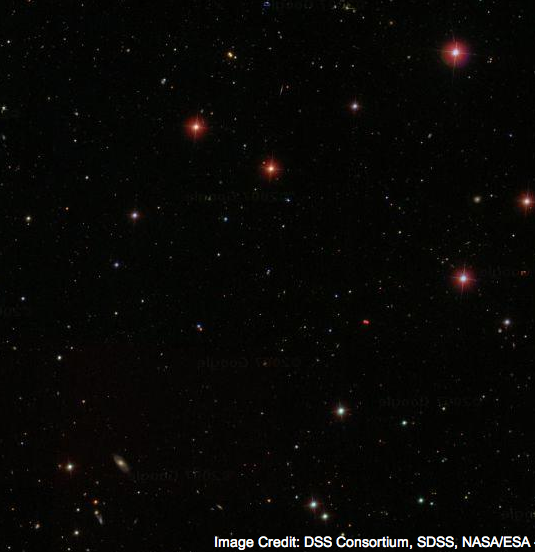
\includegraphics[height=6cm]{Sky1}\hsp
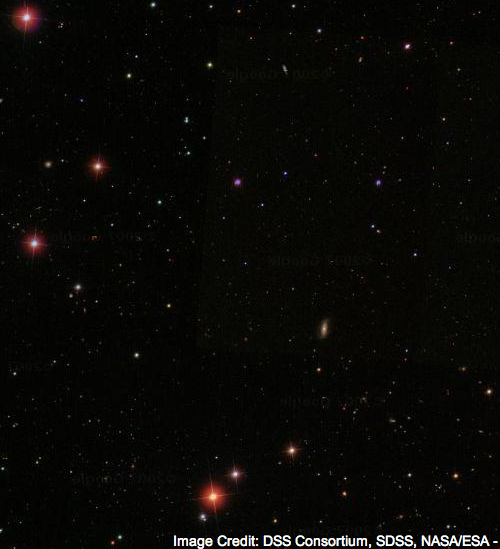
\includegraphics[height=6cm]{Sky2}\end{center}
\hspace{1.8in}
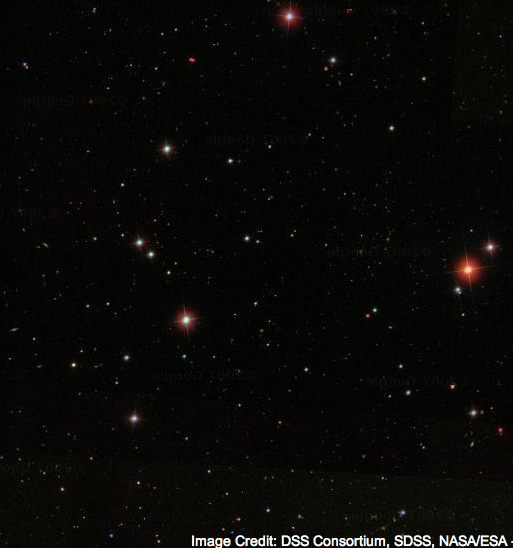
\includegraphics[height=6cm]{Sky3}}\end{center}
These are value-assignments $a_1\in\mcO(V_1), a_2\in\mcO(V_2),$ and $a_3\in\mcO(V_3)$ throughout subsets $V_1,V_2,V_3\ss X$ (respectively). These subsets $V_1,V_2,V_3$ cover some (strangely-shaped) subset $U\ss X$. The sheaf condition says that these three value-assignments glue together to form a single value-assignment throughout $U$:
\begin{center}
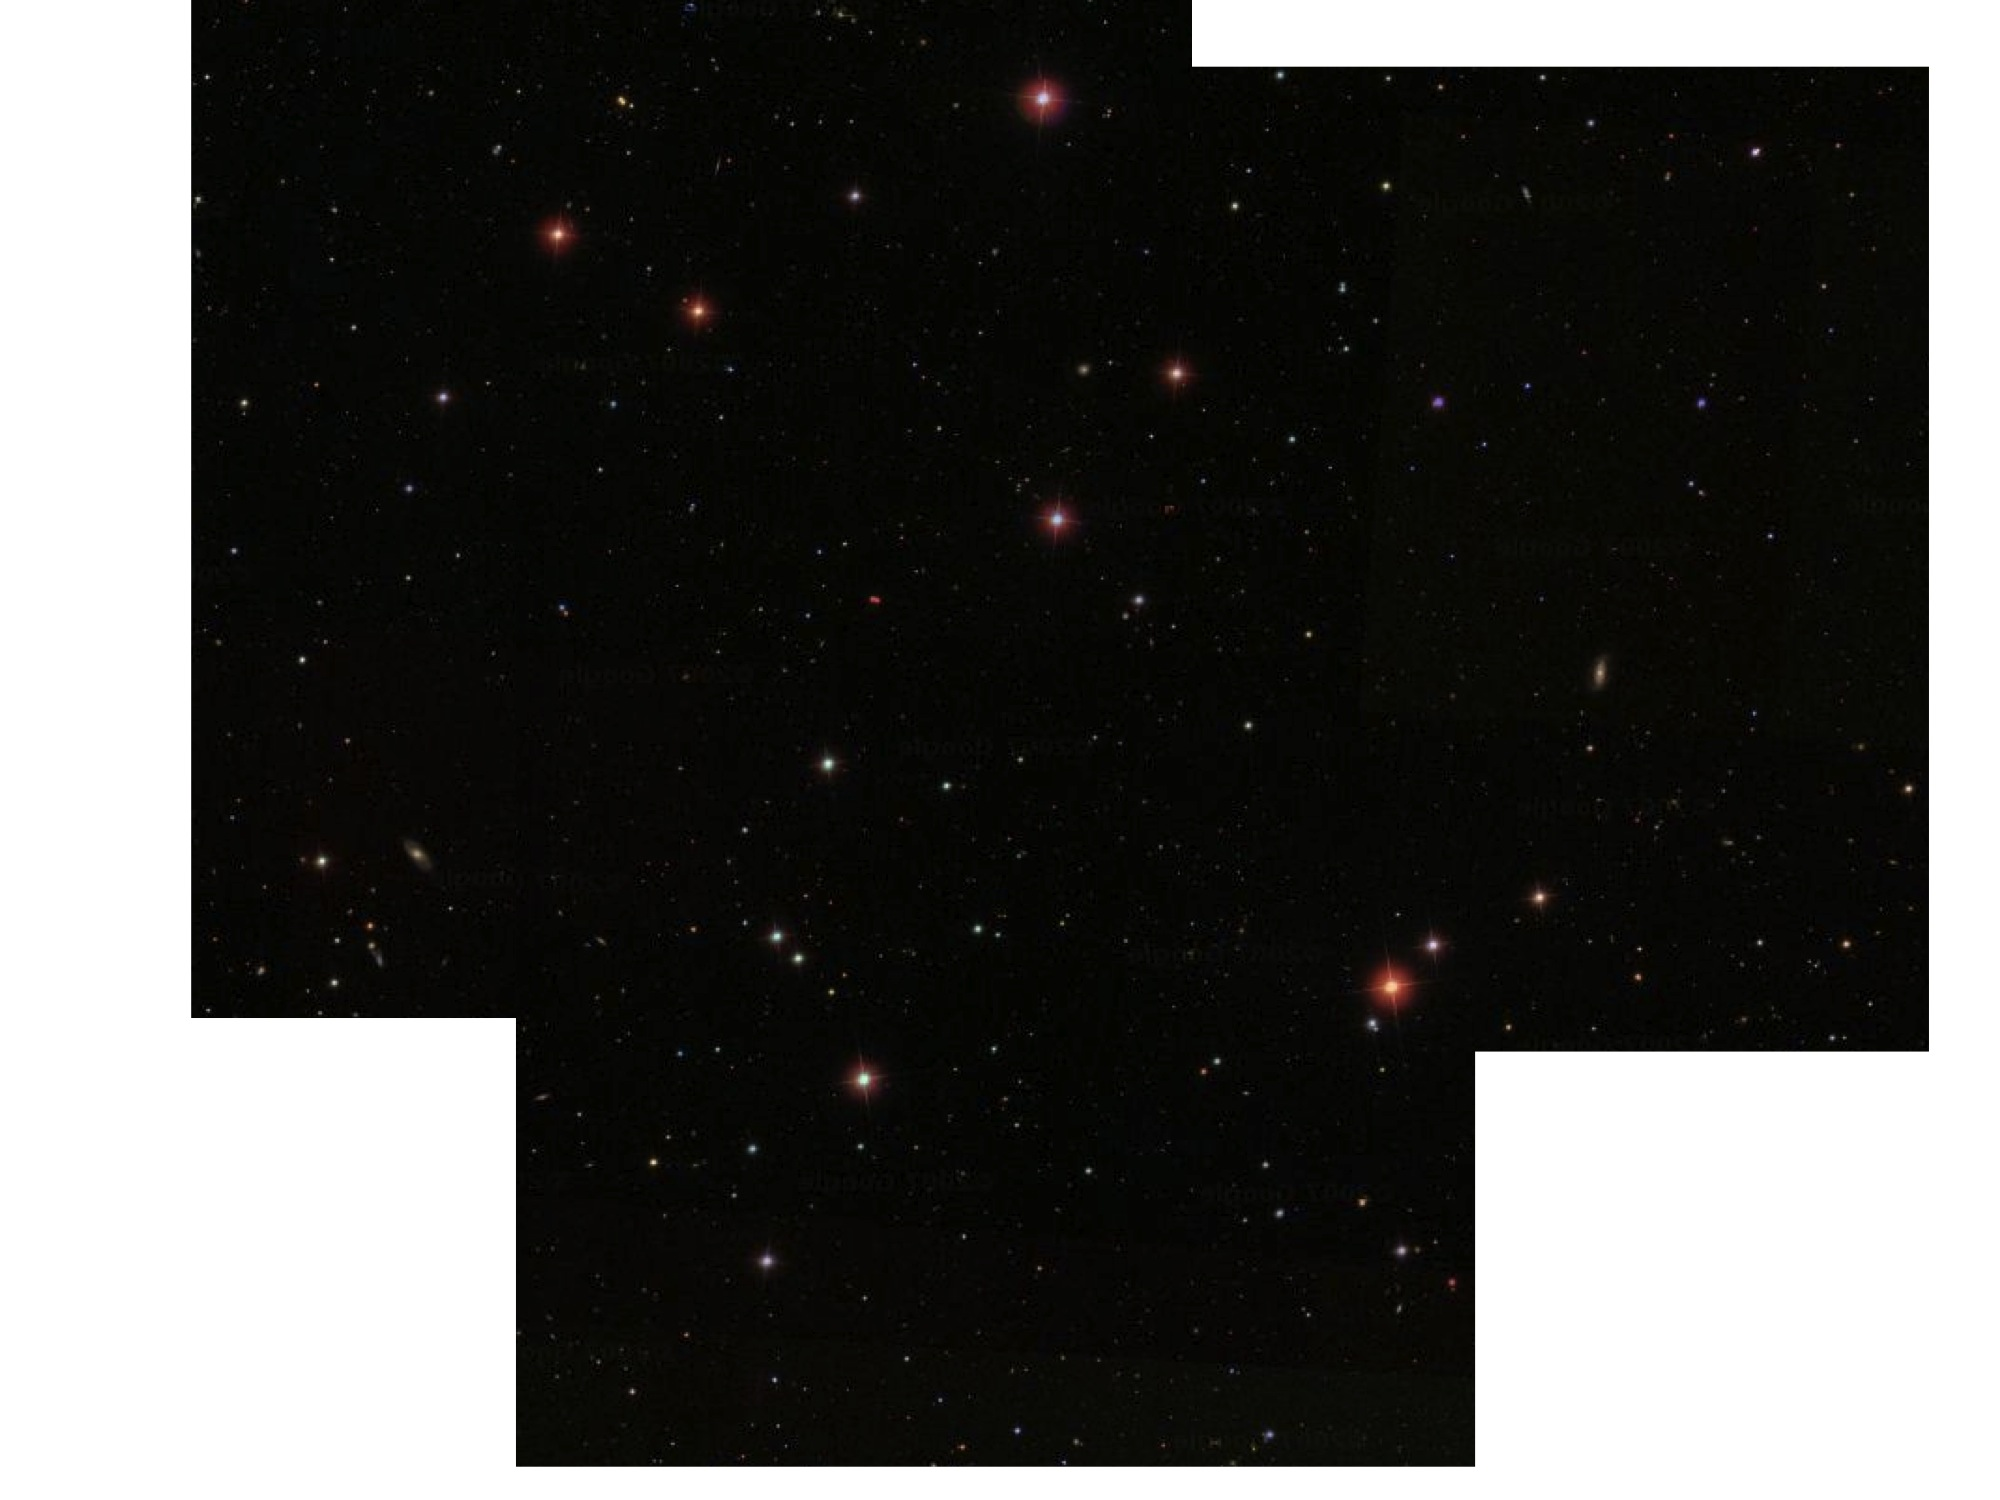
\includegraphics[height=7.5cm]{sky123}
\end{center}

\end{application}

\begin{exercise}
Find an application of sheaves in your own domain of expertise.
\end{exercise}

\begin{application}
Suppose we have a sheaf for temperatures on earth. For every region $U$ we have a set of theoretically possible temperature-assignments throughout $U$. For example we may know that if it is warm in Texas, warm in Arkansas, and warm in Kansas, then it cannot be cold in Oklahoma. With such a sheaf $\mcO$ in hand, one can use facts about the temperature in one region $U$ to predict the temperature in another region $V$. 

The mathematics is as follows. Suppose given regions $U,V\ss X$ and a subset $A\ss\mcO(U)$ corresponding to what we know about the temperature assignment throughout $U$. We take the following fiber product
$$
\xymatrix{(\rho_{U,X})^{\m1}(A)\ullimit\ar[r]\ar[d]&\mcO(X)\ar[d]^{\rho_{U,X}}\ar[r]^{\rho_{V,X}}&\mcO(V)\\
A\ar[r]&\mcO(U)}
$$
The image of the top map is a subset of $\mcO(V)$ telling us which temperature-assignments are possible throughout $V$ given our knowledge $A$ about the temperature throughout $U$.

We can imagine the same type of prediction systems for other domains as well, such as the energy of various parts of a material.
\end{application}

\begin{example}

In Exercises \ref{exc:juris 1} and \ref{exc:juris 2} we discussed the idea of laws being dictated or respected throughout a jurisdiction. If $X$ is earth, to every jurisdiction $U\ss X$ we assign the set $\mcO(U)$ of laws that are dictated to hold throughout $U$. Given a law on $U$ and a law on $V$, we can see if they amount to the same law on $U\cap V$. For example, on $U$ a law  might say “no hunting near rivers” and on $V$ a law might say “no hunting in public areas”. It just so happens that on $U\cap V$ all public areas are near rivers and vice versa, so the laws agree there. These laws patch together to form a single rule about hunting that is enforced throughout the union $U\cup V$, respected by all jurisdictions within it.

\end{example}

%% Subsubsection %%

\subsubsection{\caseENGRUS{Sheaf of ologged concepts}{ / }{Пучок концептов олога}}\index{olog!sheaf of}

Definition \ref{def:sheaf} defines what should be called a sheaf of sets. We can discuss sheaves of groups or even sheaves of categories. Here is an application of the latter.

Recall the notion of simplicial complexes discussed in Section \ref{sec:simplicial complex}\index{simplicial complex}. They look like this: 
\begin{align}\label{dia:olog network}
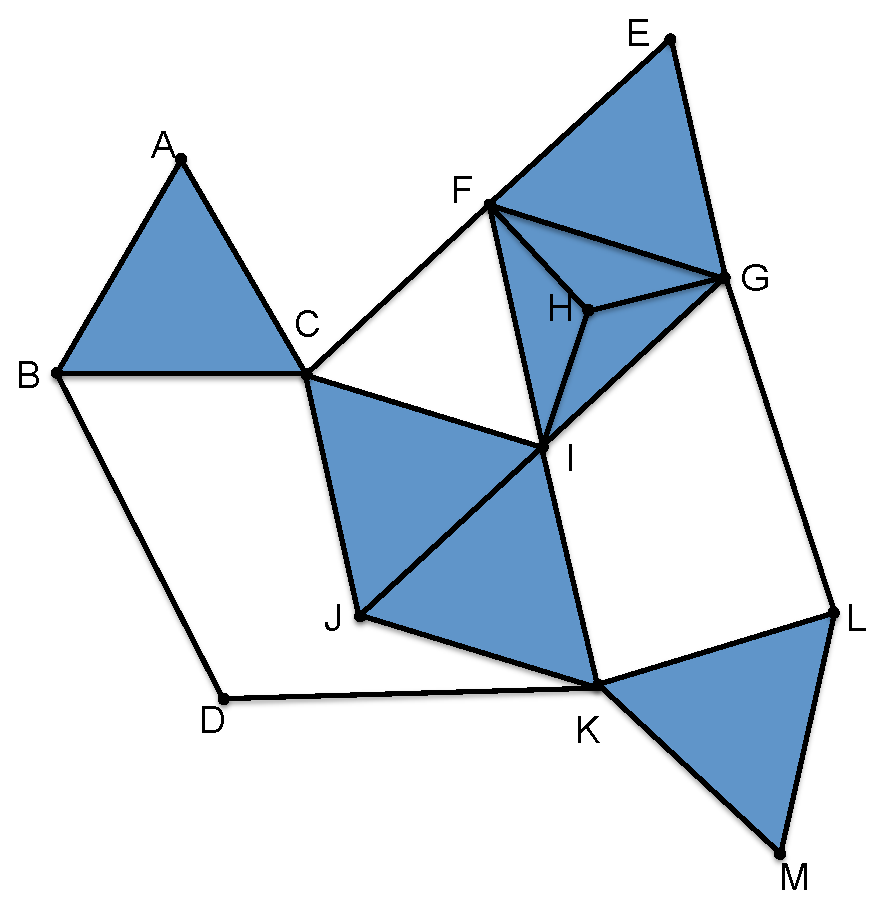
\includegraphics[height=3in]{OlogNetwork5}
\end{align} 
Given such a simplicial complex $X$, we can imagine each vertex $v\in X_0$ as an entity with a worldview (e.g. a person) and each simplex as the common worldview shared by its vertices. To model this, we will assign to each vertex $v\in X$ an olog $\mcO(v)$, corresponding to the worldview held by that entity, and to each simplex $u\in X_n$, we assign an olog $\mcO(u)$ corresponding to a {\em common ground} worldview.\index{common ground}. Recall that $X$ is a subset of $\PP(X_0)$; it is a preorder and its elements (the simplices) are ordered by inclusion. If $u,v$ are simplices with $u\ss v$ then we want a map of ologs (i.e. a schema morphism) $\mcO(v)\to\mcO(u)$ corresponding to how any idea that is shared among the people in $v$ is shared among the people in $u$. Thus we have a functor $\mcO\taking X\to\Sch$ (where we are forgetting the distinction between ologs and databases for notational convenience).

To every simplicial complex (indeed every ordered set) one can associate a topological space; in fact we have a functor $Alx\taking\PrO\to\Top$,\index{a functor!$\PrO\to\Top$} called the \href{http://en.wikipedia.org/wiki/Alexandrov_topology}{\text Alexandrov} functor. Applying $Alx(X\op)$ we have a space which we denote by $\mcX$. One can visualize $\mcX$ as $X$, but the open sets include unions of simplices. There is a unique sheaf of categories on $\mcX$ that behaves like $X$ on simplices.

How does this work in the case of our sheaf $\mcO$ of worldviews? For simplices such as $(A)$ or $(CI)$, the sheaf returns the olog corresponding to that person or shared worldview. But for open sets like the union of $(CIJ)$ and $(IJK)$, what we get is the olog consisting of the types shared by $C, I$, and $J$ for which $I$ and $J$ affirm agreement with types shared by $I, J$, and $K$.

\begin{example}

Imagine two groups of people $G_1$ and $G_2$ each making observations about the world. Suppose that there is some overlap $H=G_1\cap G_2$. Then it may happen that there is a conversation including $G_1$ and $G_2$ and both groups are talking about something and, although using different words, $H$ says “you guys are talking about the same things, you just use different words.” In this case there is an object-assignment throughout $G_1\cup G_2$ that agrees with both those on $G_1$ and those on $G_2$.

\end{example}

%% Subsubsection %%

\subsubsection{\caseENGRUS{Time}{ / }{Время}}

One can use sheaves to model objects in time; Goguen gave an approach to this in \cite{Gog}. For another approach, let $\mcC$ be a database schema. The lifespan of information about the world is generally finite; that is, what was true yesterday is not always the case today. Thus we can associate to each interval $U$ of time the information that we deem to hold throughout $U$. This is sometimes called the {\em valid time}\index{data!valid time} of the data.

If something is the case throughout $U$ and we have a subset $V\ss U$ then of course it is the case throughout $V$. And the sheaf condition holds too: if some information holds throughout $U$ and some other information holds throughout $U'$, and if these two things restrict to the same information on the overlap $U\cap V$, then they can be glued to information that holds throughout the union $U\cup V$.

So we can model information-change over time by using a sheaf of $\mcC$-sets on the topological space $\RR$. One way to think of this is simply as an instance on the schema $\mcC\times\Op(\RR)\op$. The sheaf condition is just an added property that our instances have to obey.

\begin{example}

Consider a hospital in which babies are born. In our scenario, mothers enter the hospital, babies are born, mothers and babies leave the hospital. Let $\mcC$ be the schema 
$$\fbox{\xymatrix{\obox{c}{.5in}{a baby}\LA{rr}{was birthed by}&\hspace{.2in}&\obox{m}{.6in}{a mother}}}$$
Consider the 8-hour intervals 
\begin{align*}
\tn{Shift}_1&:=(\tn{Jan }1 - 00:00,\tn{ Jan }1 - 08:00),\\
\tn{Shift}_2&:=(\tn{Jan }1 - 04:00,\tn{ Jan }1 - 12:00),\\
\tn{Shift}_3&:=(\tn{Jan }1 - 8:00,\tn{ Jan }1 - 16:00).
\end{align*}
The nurses take shifts of 8 hours, overlapping with their predecessors by 4 hours, and they record in the database only patients that were there throughout their shift or throughout any overlapping shift. A mother might be in the hospital throughout shift 1, arriving before the new year. A baby is born at 05:00 on Jan 1, and thus does not make it into the $\tn{Shift}_1$-table, but does make it into the $(\tn{Shift}_1\cap\tn{Shift}_2)$-table. The two are there until 17:00 on Jan 1, and so they are recorded in the $\tn{Shift}_2$ and $\tn{Shift}_3$ tables. 

\end{example}

Whether or not this implementation of the sheaf semantics is most useful in practice is certainly debatable. But something like this could easily be useful as a semantics, i.e. a way of thinking about, the temporal nature of data.

